\documentclass[12pt]{article}
\usepackage[parfill]{parskip}
%Mathematical TeX packages from the AMS
\usepackage{amssymb,amsmath,amsthm} 
%geometry (sets margin) 
\usepackage[margin=1.25in]{geometry}	
\usepackage{enumerate}					
\usepackage{graphicx}
\usepackage{amsfonts}
\usepackage{hyperref}
\usepackage{subfigure}

\theoremstyle{plain}% default
\newtheorem{thm}{Theorem}[section]
\newtheorem{lem}[thm]{Lemma}
\newtheorem{prop}[thm]{Proposition}

\theoremstyle{definition}
\newtheorem{defn}{Definition}[section]
\newtheorem{conj}{Conjecture}[section]
\newtheorem{exmp}{Example}[section]

\theoremstyle{remark}
\newtheorem*{rem}{Remark}
\newtheorem*{note}{Note}
\newtheorem{case}{Case}

\begingroup
    \makeatletter
    \@for\theoremstyle:=definition,remark,plain\do{%
        \expandafter\g@addto@macro\csname th@\theoremstyle\endcsname{%
            \addtolength\thm@preskip\parskip
            }%
        }
\endgroup
%=============================================================
%Fancy-header package to modify header/page numbering 
%
\usepackage{fancyhdr}
\pagestyle{fancy}
\lhead{Wesley Chen, Brandon Sim}
\chead{} 
\rhead{\thepage} 
\lfoot{\small Applied Math 120} 
\cfoot{} 
\rfoot{\footnotesize Automating Brain Tumor Detection in MRI Images} 
\renewcommand{\headrulewidth}{.3pt} 
\renewcommand{\footrulewidth}{.3pt}
\setlength\voffset{-0.25in}
\setlength\textheight{648pt}

%=============================================================

\begin{document}

\title{Automating Brain Tumor Detection in MRI Images}
\author{Wesley Chen, Brandon Sim}

\maketitle
\tableofcontents
\newpage

\section{Introduction and Motivation}

The MRI (Magnetic Resonance Imaging) is one of the most accurate and available types of medical imaging that is used to detect diseases throughout the body, ranging from severe bleeding to cancerous growths (SOURCE A).  The prevalence of MRI imaging for diagnosis is well represented by the sheer number of the expensive yet critical equipment.  In the United States, there are over 10,000 MRI machines (SOURCE B).  When a doctor administers an MRI imaging (for the scope of this paper, we will be using the brain as the ordgan of study), the machine stores many 2D slices of the brain from multiple angles to provide the most accurate 3D image.  From this collection of slices, the doctor must look through each frame for possible irregularities that could confirm the existence of a tumor.  The person reading the MRI image must flip through each frame systematically – there is no shortcut to knowing about where a tumor could be.  Often times, the doctor must look at the same images multiple times even if her oe she does not see a tumor just to make sure a small tumor (which could be as large as just spanning 3 frames) was not missed.  The requirement of such a methodical but tedious search inspired us to develop approaches to automate the reading of a set of MRI images.  For the scope of this project, we explored a couple independent techniques to identify possible tumor candidates from a given 2D image (one slice of the brain).  We then extended this search to an entire stack of images represetig the full 3D brain.  Although we recognize that our algorithm will probably not fully replace a doctor's screening of MRIs, for liability and lawsuit reasons, we do hope that it will both reduce the subset a doctor has to look through, as well as be able to point out likely tumor candidates that the doctor could have missed.

\section{Methodology}

We were given a complete data set of a MRI brain scan for one patient with a relatively small tumor, courtesy of Dr. Steven Shufflebeam of Massachusetts General Hospital.  Using a small tumor as our test case, we believe that larger tumors will only be more obvious to identify.
We tried two independent approaches to ideentifying a positive tumor case out of a given 2D frame: the first was using watershed segmentation to filter various foreground objects – hoping to identify the tumor as one of the fewer remaining objects.  A brain tumor usually appears as a denser, white area which should be filtered out by the segmentation algorithm.  Because this algorithm relies on 3D detail which our 2D scan did not have, we tried a simpler, more elegant method, 2D-limited strategy.

The second method we used was based on a symmetry analysis algorithm.  A tumor should be recognized as a closed object in our image.  We could identify this closed region from an edge detection step.  Then, we wanted to use the natural symmetry of the brain to detect the tumor.  A tumor would be an irregular growth and would not have a symmetric counterpart.

If either method worked, we would save the 3D location (using the frame number).  We woudl then check which tumor candidates came up consistent across several consecutive frames - and these would be identified by our final program output.
\subsection{Watershed Segmentation}

The goal of the watershed segmentation method is to map the image to a topological equivalent, and “flood out” various “basins” to represent different levels of foreground.  The first step would be to convert to grayscale.  The intensity of the grayscale code would be mapped to relative height.  Conceptually, once this grayscale mapping is complete, the “whitest” pixels would represent areas of maximum height (or intensity or density in the case of an MRI image).  Using a gradient magnitude should result in proper segmentation.  However, due to small differences in gradient, this results in an overly segmented product (see results section below).

To eliminate such detail, a set of image erosion and dilations must be conducted to eliminate some foreground detail.  The foreground is selected through a morphological structuring element provided by the strel() function of Matlab’s image processing toolkit.  We chose to use “disk” shaped elements as the round object best represents the structures we would find in the brain.  We then calibrated the size of this element and this is where we controlled the level of segmentation.  This element is used by the image manipulation functions below.

After this element is created, we used other Matlab image processing functions (namely imerode() and imdilate() ) to help remove foreground detail and provide a map of topological height “most prominent foreground areas.”  Imerode() and imdilate() are complimentary functions that look at every subset of the disk shaped element within the full image matrix to find areas with very similarly colored pixels – combining them into a gradual gradient.  In other words, it dilates the detail of the foreground to produce more uniform areas that won’t over-segment when running a watershed algorithm. 

After the establishment of the foreground markers, the markers were superimposed over the original image.  Another sequence of erosion-dilation was applied to help smooth out the foreground markers superimposed onto the original image.  Then, a grayscale thresholding function was run to select the background areas.  Anything darker than a certain threshold would be marked as “background”.  Then, the watershed() function was called to create ridges (the valleys of the basin area – also our background).  This background marker image was then superimposed onto the image with the foreground marker to create the fully marked image.  In our MRI case, because the background is uniformly black, this step was not necessary but was kept in our program for comprehensiveness (will still work on any image).

Finally, we visualized the result by using a colored watershed visualization which filled each object with a different color.  This color map was then superimposed with a 50% transparency over our original image.  Then, each color would be a different component to identify as a possible tumor candidate.
	
\subsection{Symmetry Analysis}

The first step to edge detection involved picking an edge detection algorithm.  We found various edge detection algorithms including Canny and Sorbel methods.  Canny is generally considered to be the more optimal algorithm.  It uses hystresis tresholding over a fixed threshold and this allows the algorithm to be more robust to noise, provide thinner edge lines and avoid treating 1 thicker edge as 2 separate ones (SOURCE C).  

Mention smoothing, thresholds

DID YOU WANT TO TALK ABOUT RANKING THE AREAS?

The dude’s edge list library – CITE BELOW

\subsection{Expansion to Full Image Set}

Region functions like the ellipse things

CENTROID,

TALK ABOUT THE MULTIPLE SLICES HERE

\section{Results}

\subsection{Watershed Segmentation}

For both cases, we started with the 2D MRI snapshot below that we selected from the stack as it clearly shows the tumorw - the white area located in the bottom left quandrant.

\begin{figure}[!h]
	\centering
		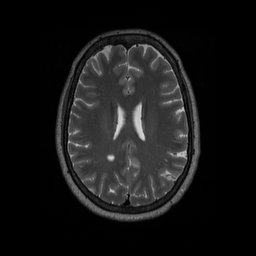
\includegraphics{original.jpg}
	\caption{Original 2D Tumor Image}
\end{figure}

Because the watershed segmentation algorithm is designed for more complex (3D), we will also show the output for a given colored image, this lily pad landscape.

\subsection{Symmetry Analysis}

\subsection{Expansion to Full Image Set}

\begin{figure}[!h]
	\centering
		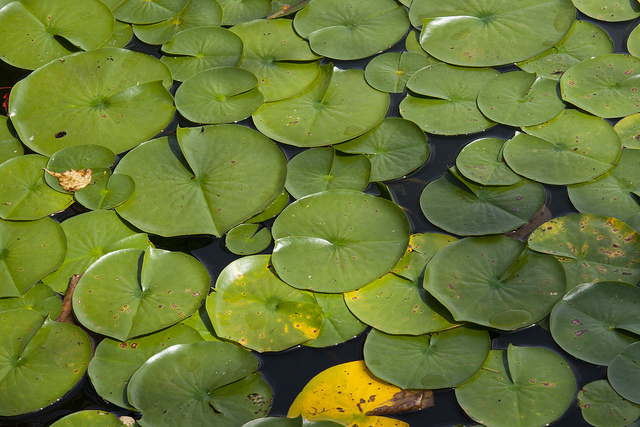
\includegraphics{lilypad.jpg}
	\caption{Original Lilypad Landscape}
\end{figure}

\section{Discussion and Future Work}

\section{Conclusion}
In conclusion, we...(talk about what we did, general overview stuff that we said in the presentation - how we combined two methods, one more traditional method, one more specific to our application, etc, etc)

We invite you to view all of our code at \url{https://github.com/bksim/images}.
\section{References}
\begin{enumerate}
\item MATLAB - image processing toolbox
\item 

\end{enumerate}
	
\section{Appendix A: Watershed Segmentation Images}
% how to include graphics (put all images in same folder)‎
\begin{figure}[!h]
	\centering
		\mbox{\subfigure[Caption1]{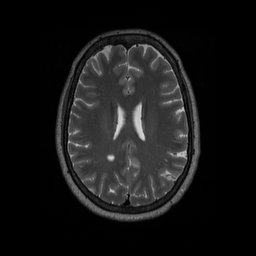
\includegraphics[width=0.45\textwidth]{original.jpg}}\quad
		\subfigure[Caption2]{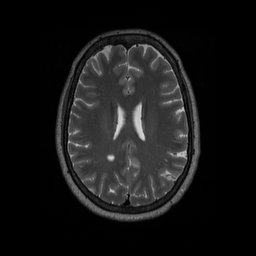
\includegraphics[width=0.45\textwidth]{original.jpg}}}
\end{figure}

\section{Appendix B: Symmetry Analysis Images}

\section{Appendix C: MATLAB code}
\subsection{Watershed Segmentation Code}
Treats the input image across various filters to display the final watershed segmented color overlay.
\subsubsection{filename.m}
\begin{verbatim}
code here
\end{verbatim}

\subsection{Symmetry Analysis Code}
Description of what file does.
\subsubsection{filename.m}
\begin{verbatim}
code here
\end{verbatim}

\subsection{Anomaly Detection Code}
Description of what file does.
\subsubsection{filename.m}
\begin{verbatim}
code here
\end{verbatim}

\subsection{Miscellaneous Code}
Converts stack of MRI images stored as a GIF into a sequence of JPEG files
\subsubsection{python.py}
\begin{verbatim}
code here
\end{verbatim}
\end{document}